\chapter{Sistem de dialog}

% todo: citari de sericii si lucrari

Construcția unui agent virtual menit să întrețină cursul unei conversații a fost întotdeauna un etalon al performanței de cercetare, de aceea testul ce poartă numele cercetătorului britanic Alan Turing \ref{test-turing} a fost pană de curând un criteriu în această direcție.

Au fost propuse diferite arhitecturi și moduri de a schița matematic o conversație, printre ele și ELIZA compus dintr-un set de reguli elaborate pe baza mai multor studii având la bază logica. Bineînțeles industria cere și abordări mai modulare, mai robuste dar care să nu iasă din tipare, în această direcție făcându-și apariția prima arhitectură bazată pe umplerea de sloturi (GUS), adică pentru fiecare replică din dialog se extrag constituenți semantici specifici domeniului care mai apoi sunt completați într-o structură tabelară (frame) urmând să servească drept parametrii în interogările cu sistemul.

Dacă privim la scopul final al unei conversații distingem două clase și anume: agenți orientați pe rezolvarea de cerințe și agenți orientați pe discuție la nivel general.

Cum majoritatea asistenților virtuali sunt dezvoltați în scopuri comerciale, rezolvarea cerințelor primează în funcționalitatea unei astfel de aplicații, așadar industria se concentrează pe arhitecturi modulare care să necesite cât mai puține date de antrenare, RASA, SNIPS, WATSON, DialogFlow sunt platforme care pun la dispoziție instrumente pentru a crea genul acesta de agenți.

Prin natura sa lumea academică explorează noi metode de a gestiona un dialog, iar acum cele mai populare abordări se concentrează pe dezvoltarea unui singur model care să descopere strategii de a acționa în diferite situații, mai exact se folosesc rețele neurale recurente pentru a capta contextul unei replici și pentru a genera răspunsuri, iar pentru a reprezenta contextul conversației și a genera politici de decizie se folosește învățarea prin recompensă. \cite{rl-seq2seq}

În cadrul studiului curent accentul este pus pe structura ce îmbină mai multe modele, drept pentru care vor fi detaliate experimentele ce au condus la alegerea unui model care să înțeleagă textul (NLU).

\section{Înțelegerea limbajului natural}
\begin{figure}[h]
	\centering
	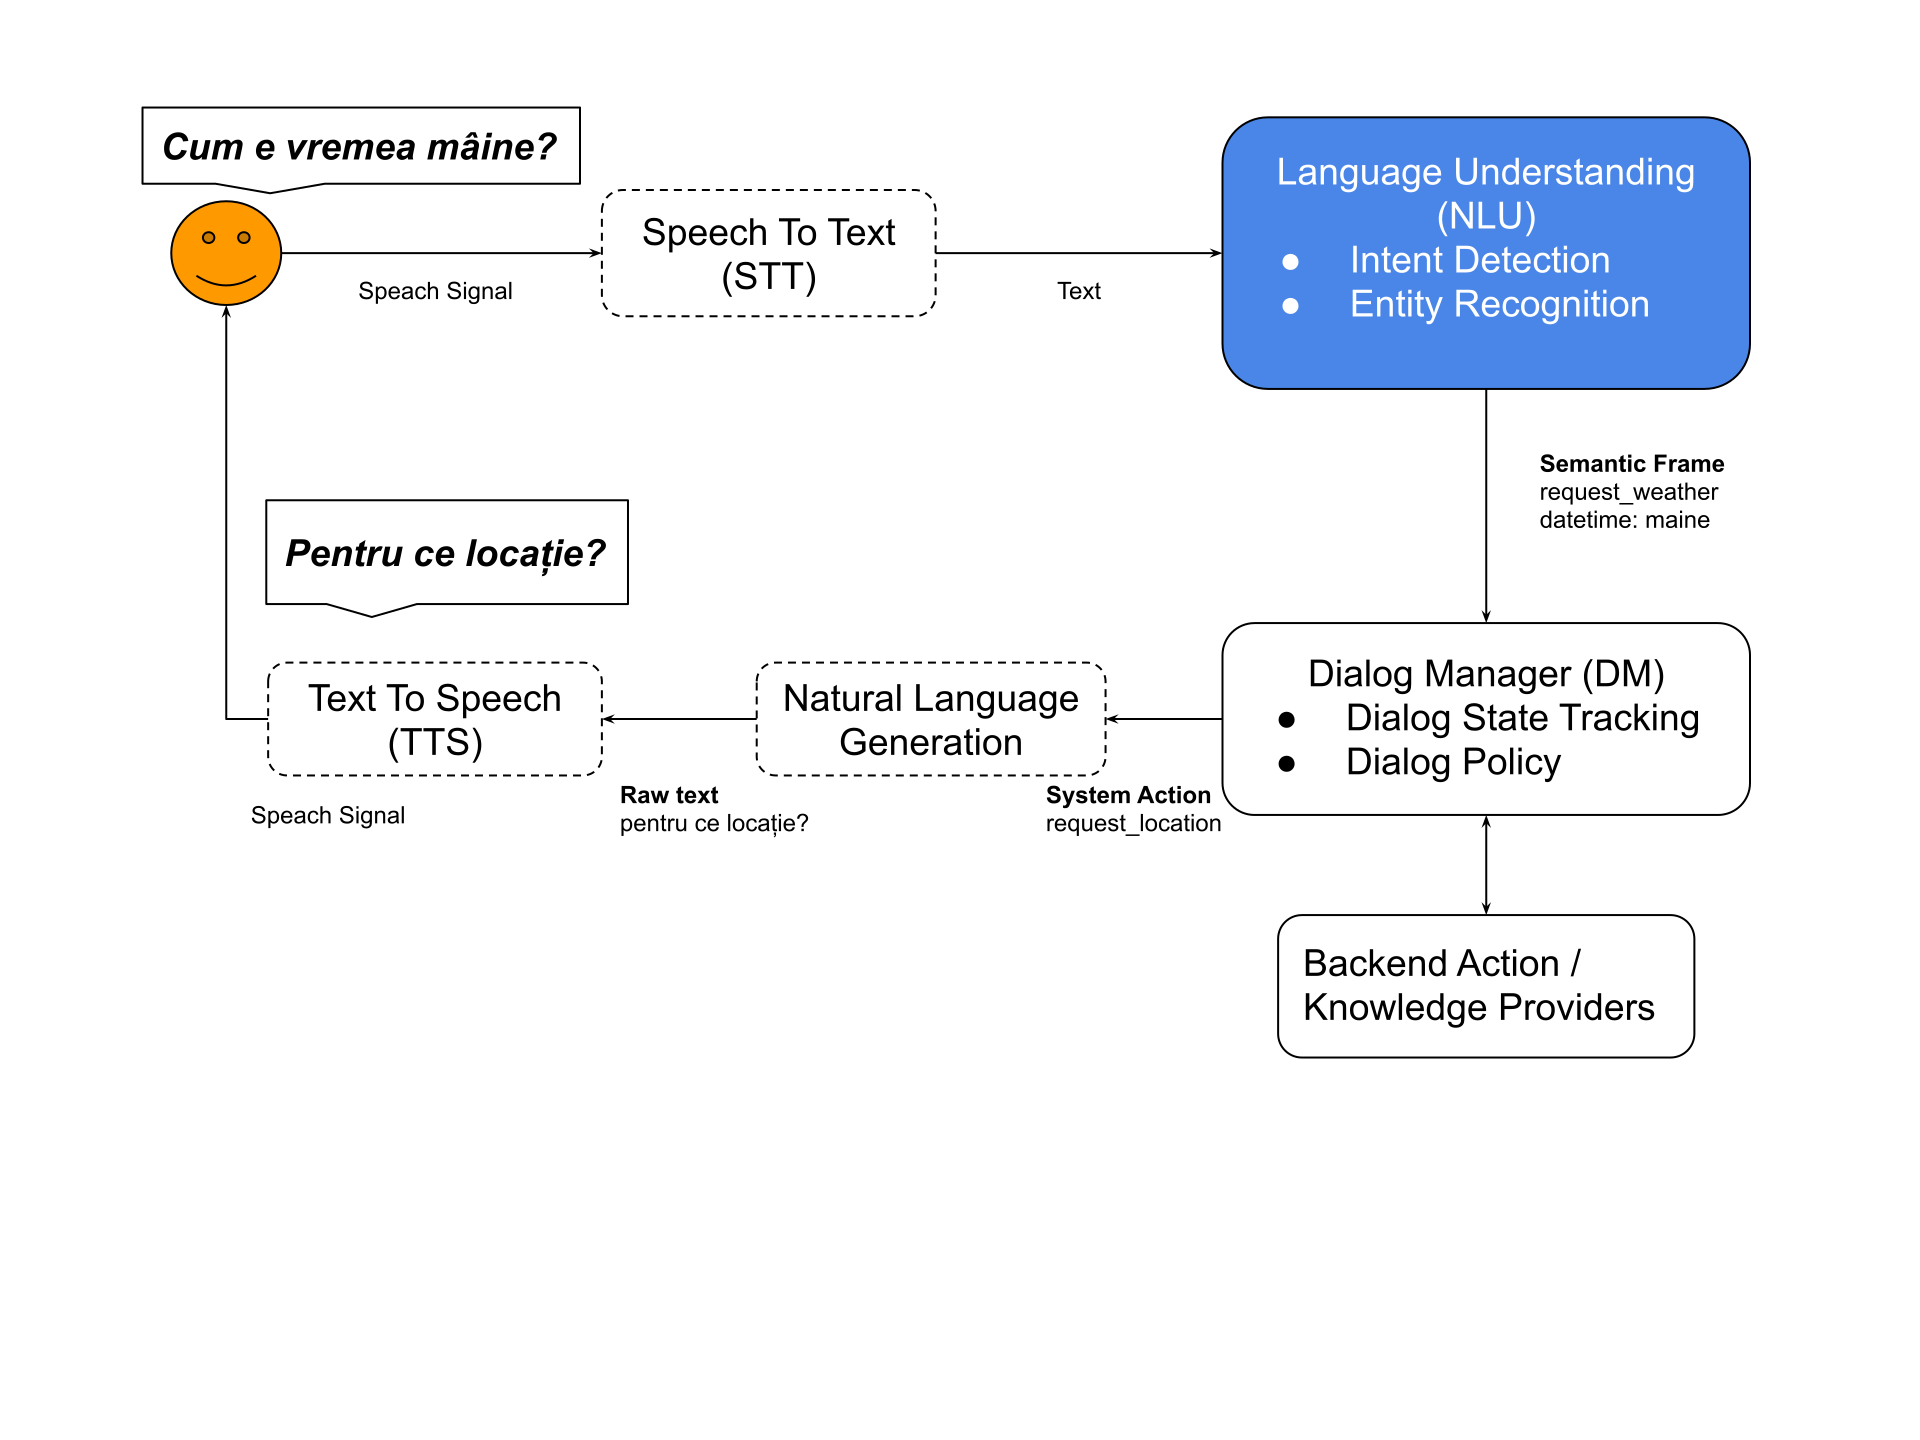
\includegraphics[scale=0.3]{nlu_dialog_system.png}
	\caption{Administrator de dialog}
	\label{fig:nlu_ds_proc}
\end{figure}
NLU este un concept destul de vast, in terminologia sistemelor de dialog acesta joacă rolul componentei care detectează intenția vorbitorului si extrage constituenți semantici din limbajul natural exprimat.
Detecția intenției poate fi tratata ca o problema de clasificare a unei replici din punct de vedere semantic, iar recunoașterea entităților poate fi văzută ca o etichetare de secvențe.
\subsection{Abordări anterioare}

% todo: de citat lucrarile

Pentru detectarea intenției se pot folosi tehnici standard de clasificare a unui text si anume SVM (Haffner et al., 2003), dar si rețele neurale convoluționale (CNNs) (Xu and Sarikaya, 2013) întâlnite adesea în procesarea imaginilor.

Pentru recunoașterea entităților se folosesc abordări precum (MEMMs) (McCallum et al., 2000), conditional random fields (CRFs) (Raymond and Riccardi, 2007), și rețele neurale recurente (RNNs) (Yao et al., 2014; Mesnil et al., 2015)

Având la baza înțelegerea limbajului, majoritatea lucrărilor actuale se concentrează pe rezolvarea concomitenta a acestor doua probleme, întrucât combinarea celor doua modele ajuta la învățarea unei reprezentări cat mai precise a textului. \cite{joint models-attention models}


\subsection{Model propus}

Rețelele neuronale recurente (RNN) sunt unele dintre cele mai populare modele matematice folosite în procesarea limbajului natural, avantajul pe care acestea îl oferă se datorează într-o mare măsură formelor sale LSTM, GRU, dar și prin caracterul lor de a învăța din date cu caracter secvențial. Aceste tipuri de rețele sunt folosite adesea ca structuri de bază pentru a crea alte modele de calcul, un exemplu este rețeaua de codificare-decodificare (seq2seq), formată din două rețele recurente, una pentru captarea (codarea) înțelesului unei secvențe iar cealaltă pentru operația de decodificare într-o secvență de ieșire.

Modelul propus pentru înțelegere a limbajului rezolvă ambele probleme simultan folosind un codificator pentru reprezentarea înțelesului unei propoziții și două decodificatoare câte unul pentru fiecare chestiune. Figura \ref{fig:seq2seq_x} sintetizează procesele implicate în acest model.

\begin{figure}[htbp]
	\centering
	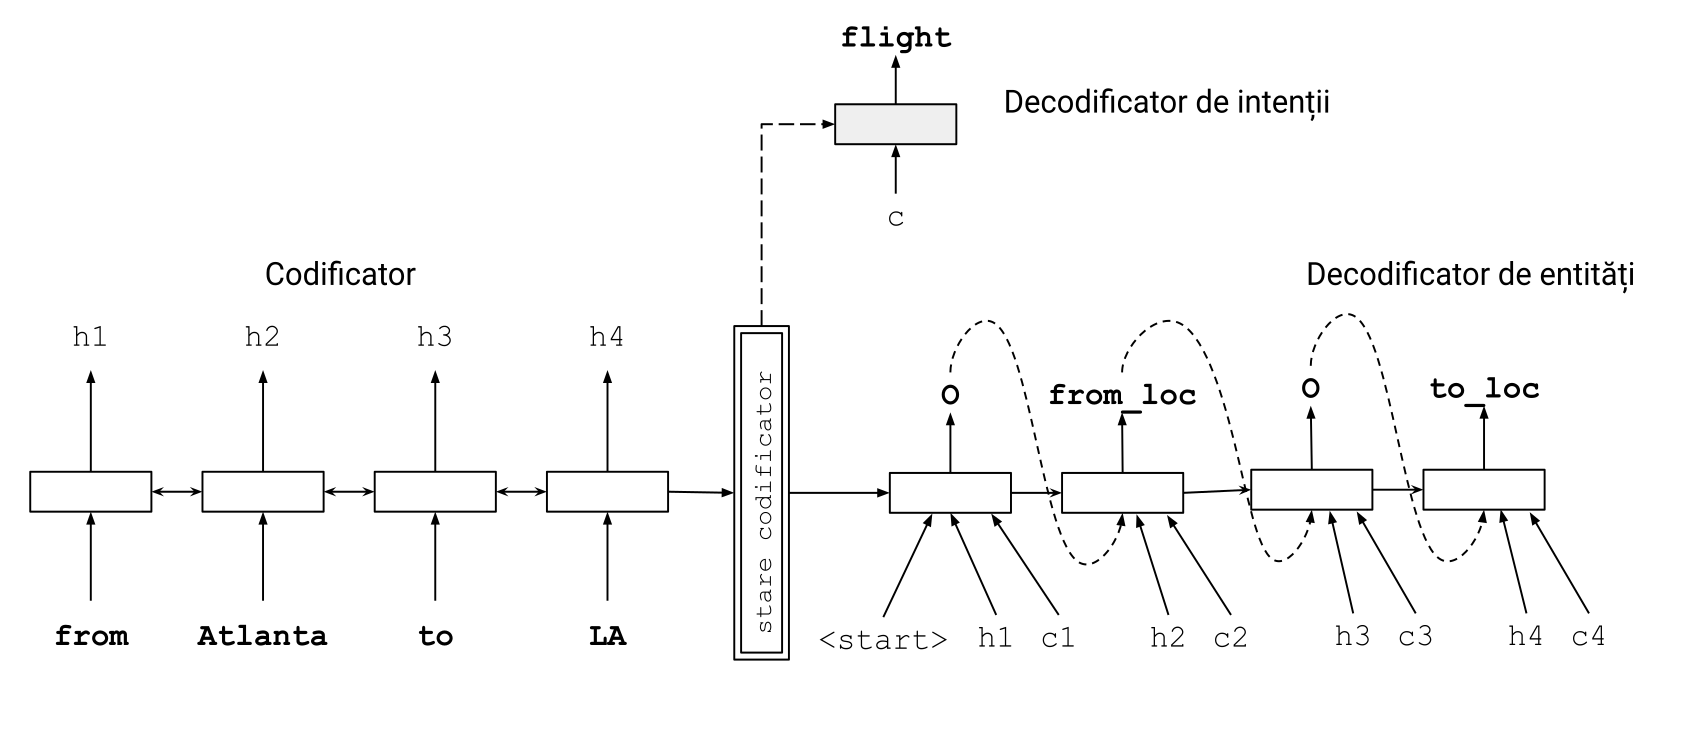
\includegraphics[scale=0.33]{seq2seq_x.png}
	\caption{Seq2Seq-x}
	\label{fig:seq2seq_x}
\end{figure}

Pentru recunoașterea entităților se dorește etichetarea unei secvențe de cuvinte $ x= (x_1, ..., x_T)$ într-o altă secvență de nume de entități corespunzătoare $ y=(y_1, ..., y_T) $. Operația de codificare se realizează prin citirea întregii secvențe de către o rețea recurentă bidirecțională, înțelesul secvenței de intrare este reprezentat de suma celor două stări ascunse finale, adică pentru citirea de la stânga la dreapta obținem stările ascunse $(fh_1, ..., fh_T)$ și invers $(bh_T, ..., bh_1)$, apoi suma celor două $h_i = [fh_i + bh_i]$ este folosită drept codificare a înțelesului secvenței de intrare. Alte lucrări \cite{joint_online_bing} folosesc ca stare ascunsă finală $h_i$ o concatenare a celor două stări. Alegerea de a aduna cele două reprezentări în schimbul concatenării, ține de faptul că dimensiunea reprezentării finale crește în cazul concatenării, fiind mai dificil de antrenat, dublând în acest caz și jumătate din parametrii rețelei. Figura \ref{fig:enc_module} descrie procesul de codificare.

\begin{figure}[h]
	\centering
	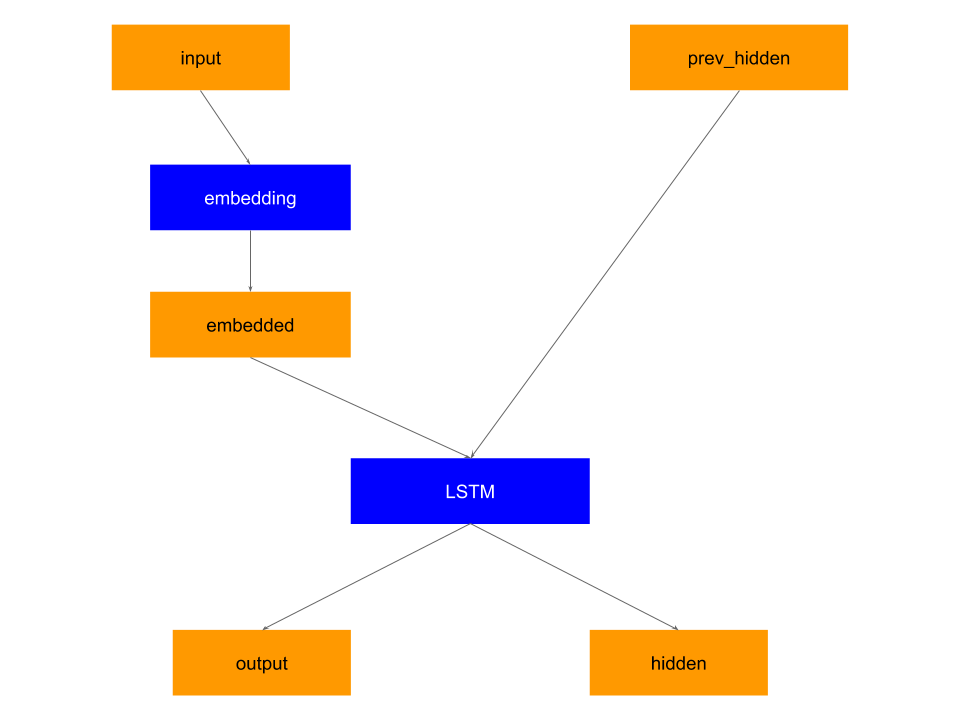
\includegraphics[scale=0.35]{encoder_module.png}
	\caption{Bidirectional Encoder}
	\label{fig:enc_module}
\end{figure}

Vom folosi reprezentarea captată de codificator pentru a inițializa operația de decodificare, aceasta este produsă de către o rețea recurentă unidirecțională, văzută ca o funcție $s_i=f(s_{i-1}, y_{i-1}, h_i, c_i)$ care la fiecare pas $i$, calculează o nouă stare $s_i$, bazată pe: starea anterioară a decodificatorului $s_{i-1}$, eticheta anterior prezisă, $y_{i-1}$, starea ascunsă din codificator corespunzătoare pasului curent, $h_i$ și un vector de context $c_i$, calculat ca o sumă ponderată peste stările ascunse din codificator.
Inspirat din \cite{trans_luong_manning} am experimentat mai multe modele de atenție.
$$ c_i = \sum_{j=1}^{T} \alpha_{i,j} h_j$$
$$ \alpha_{i,j} = \frac{\exp(score_{i, j})}{\sum_{k=1}^{T} \exp(score_{i, k})}$$

\[ score(i, k) = g(s_{i-1}, h_k) =
\begin{cases}
s_{i-1}^\top h_k			&	\quad \text{dot}\\
s_{i-1}^\top W_a h_k	&	\quad \text{general}\\
v_a^\top \tanh(W_a [s_{i-1};h_k])	&	\quad \text{concat}\\
\end{cases}
\]

Modelul de atenție poate fi văzut ca o rețea de tip feed-forward $g(s_{i-1}, h_k)$, care la fiecare pas din operația de decodare calculează ponderile pentru stările ascunse ale codificatorului, folosindu-se de ultima stare ascunsă din decodor, $s_{i-1}$ și stările ascunse $(h_1, ..., h_T)$. Mai jos în figura \ref{fig:dec_bah} este descris întreg fluxul de date și operații realizate de decodorul responsabil de etichetarea entităților.

\begin{figure}[h]
	\centering
	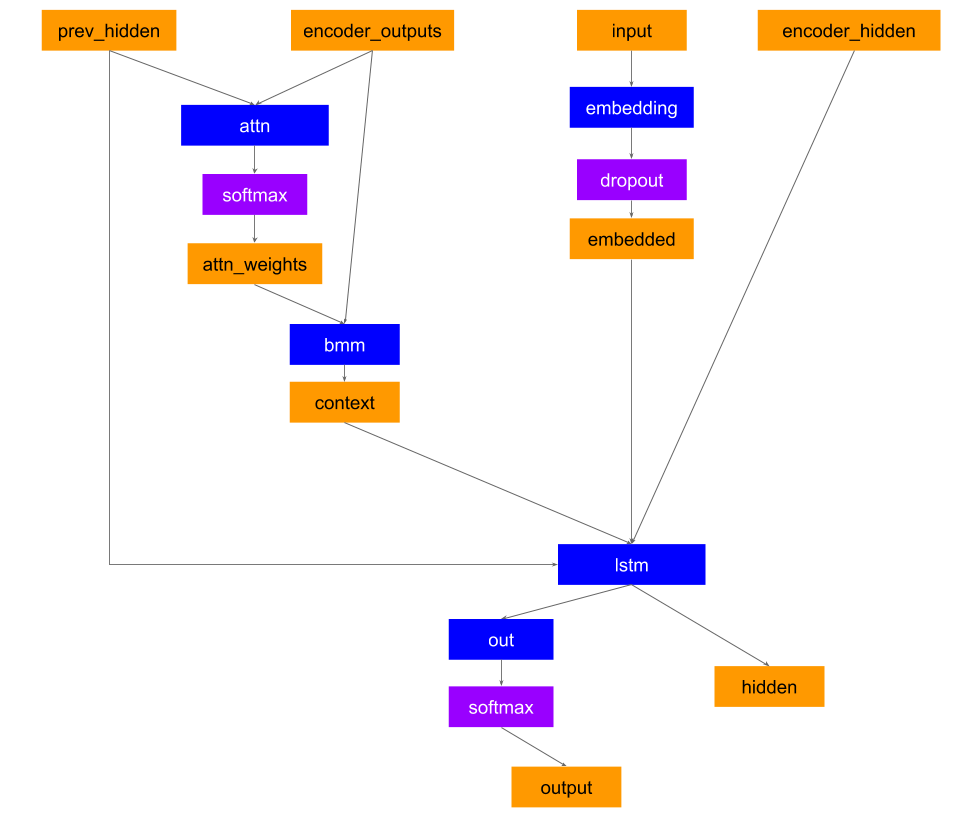
\includegraphics[scale=0.35]{decoder_bahdanau.png}
	\caption{Attention Decoder}
	\label{fig:dec_bah}
\end{figure}

%%%%%%%%%%%%%%%%%%%%%%%%%
\subsection{Mulțimea de antrenare}
ATIS (Airline Travel Information Systems) \cite{atis} este o colecție de cereri venite din partea clienților referitor la zborurile aeriene de la începutul anilor 90. DARPA este instituția americana ce s-a ocupat de colectarea acestor date. Mulțimea de antrenare conține un număr de aproape 5000 de propoziții etichetate cu intenții si entități. Formatul de etichetare utilizat este IOB (Inside–outside–beginning), care ajuta la etichetarea entitatilor formate din mai multe cuvinte, astfel încât fiecare etichetă este precedata de B-<nume-eticheta> pentru început, iar cu I-<nume-eticheta> pentru următoarele cuvinte care fac parte din entitate. Exemplele sunt date în limba engleză, iar lungimea medie a unei prepoziții este de 15 cuvinte.

\begin{table}
	\centering
	\caption{Exemplu din mulțimea de antrenare}
	\label{atis_example}
	\begin{adjustbox}{max width=\textwidth}
		\begin{tabular}{ |c|c|c|c|c|c|c|c|c|c| } 
			\hline
			\textbf{Propoziție} & flights & from & New & York & to & Cicago & on & wednesday & morning \\ 
			\hline
			\textbf{Entități} & O & O & B-from.loc & I-from.loc & O & B-to.loc & O & B-depart.day-name & B-depart.day-mood \\
			\hline
			\textbf{Intenție} & \multicolumn{8}{c}{flight} &  \\ 
			\hline
		\end{tabular}
	\end{adjustbox}
\end{table}

\begin{table}
	\centering
	\caption{Statistici ATIS}
	\label{atis_stats}
	\begin{adjustbox}{max width=\textwidth}
		\begin{tabular}{ |c|c|c|c|c|c|c| } 
			\hline
			\textbf{Multime de antrenare} & \#Train & \#Dev & \#Test & $|V|$ & \#Intenții & \#Entități \\ 
			\hline
			ATIS & 4978 & - & 893 & 900 & 22 & 80 \\
			\hline
		\end{tabular}
	\end{adjustbox}
\end{table}


%%%%%%%%%%%%%%%%%%%%
\subsection{Rezultate}
\begin{center}

	\begin{table}
		\caption{Comparație cu abordări anterioare. Antrenare independentă pentru detectarea intenției pe ATIS}
		\label{rezultate}
		\begin{tabular}{ c c c } 
			\hline
			\textbf{Model} 		 & \textbf{Scor F1 (entități)} & \textbf{Scor F1 (intenții)}\\
			\hline
			Seq2SeqX (dot - attn) & 97,5 & 96,5 \\
			\hline
			Seq2SeqX (general - attn) & 96.6 & 96,5 \\
			\hline
			Seq2SeqX (concat - attn) & 97.53 & - \\
			\hline
			Seq2SeqX (no - attn) & 97.8 & - \\
			\hline
			Seq2SeqX (no - attn, concat - attn) & 97.4 & 96.0 \\
			\hline
			Seq2SeqX (concat - intent attn) & 97.55 & 96.53 \\
			\hline
		\end{tabular}
	\end{table}
\end{center}

\subsection{Analiza erorilor}


%%%%%%%%%%%%%%%%%%%%%%%%%%%%%%%%%%%%%%%%%%%%%%%5
\section{Administrator de dialog}
\begin{figure}[h]
	\centering
	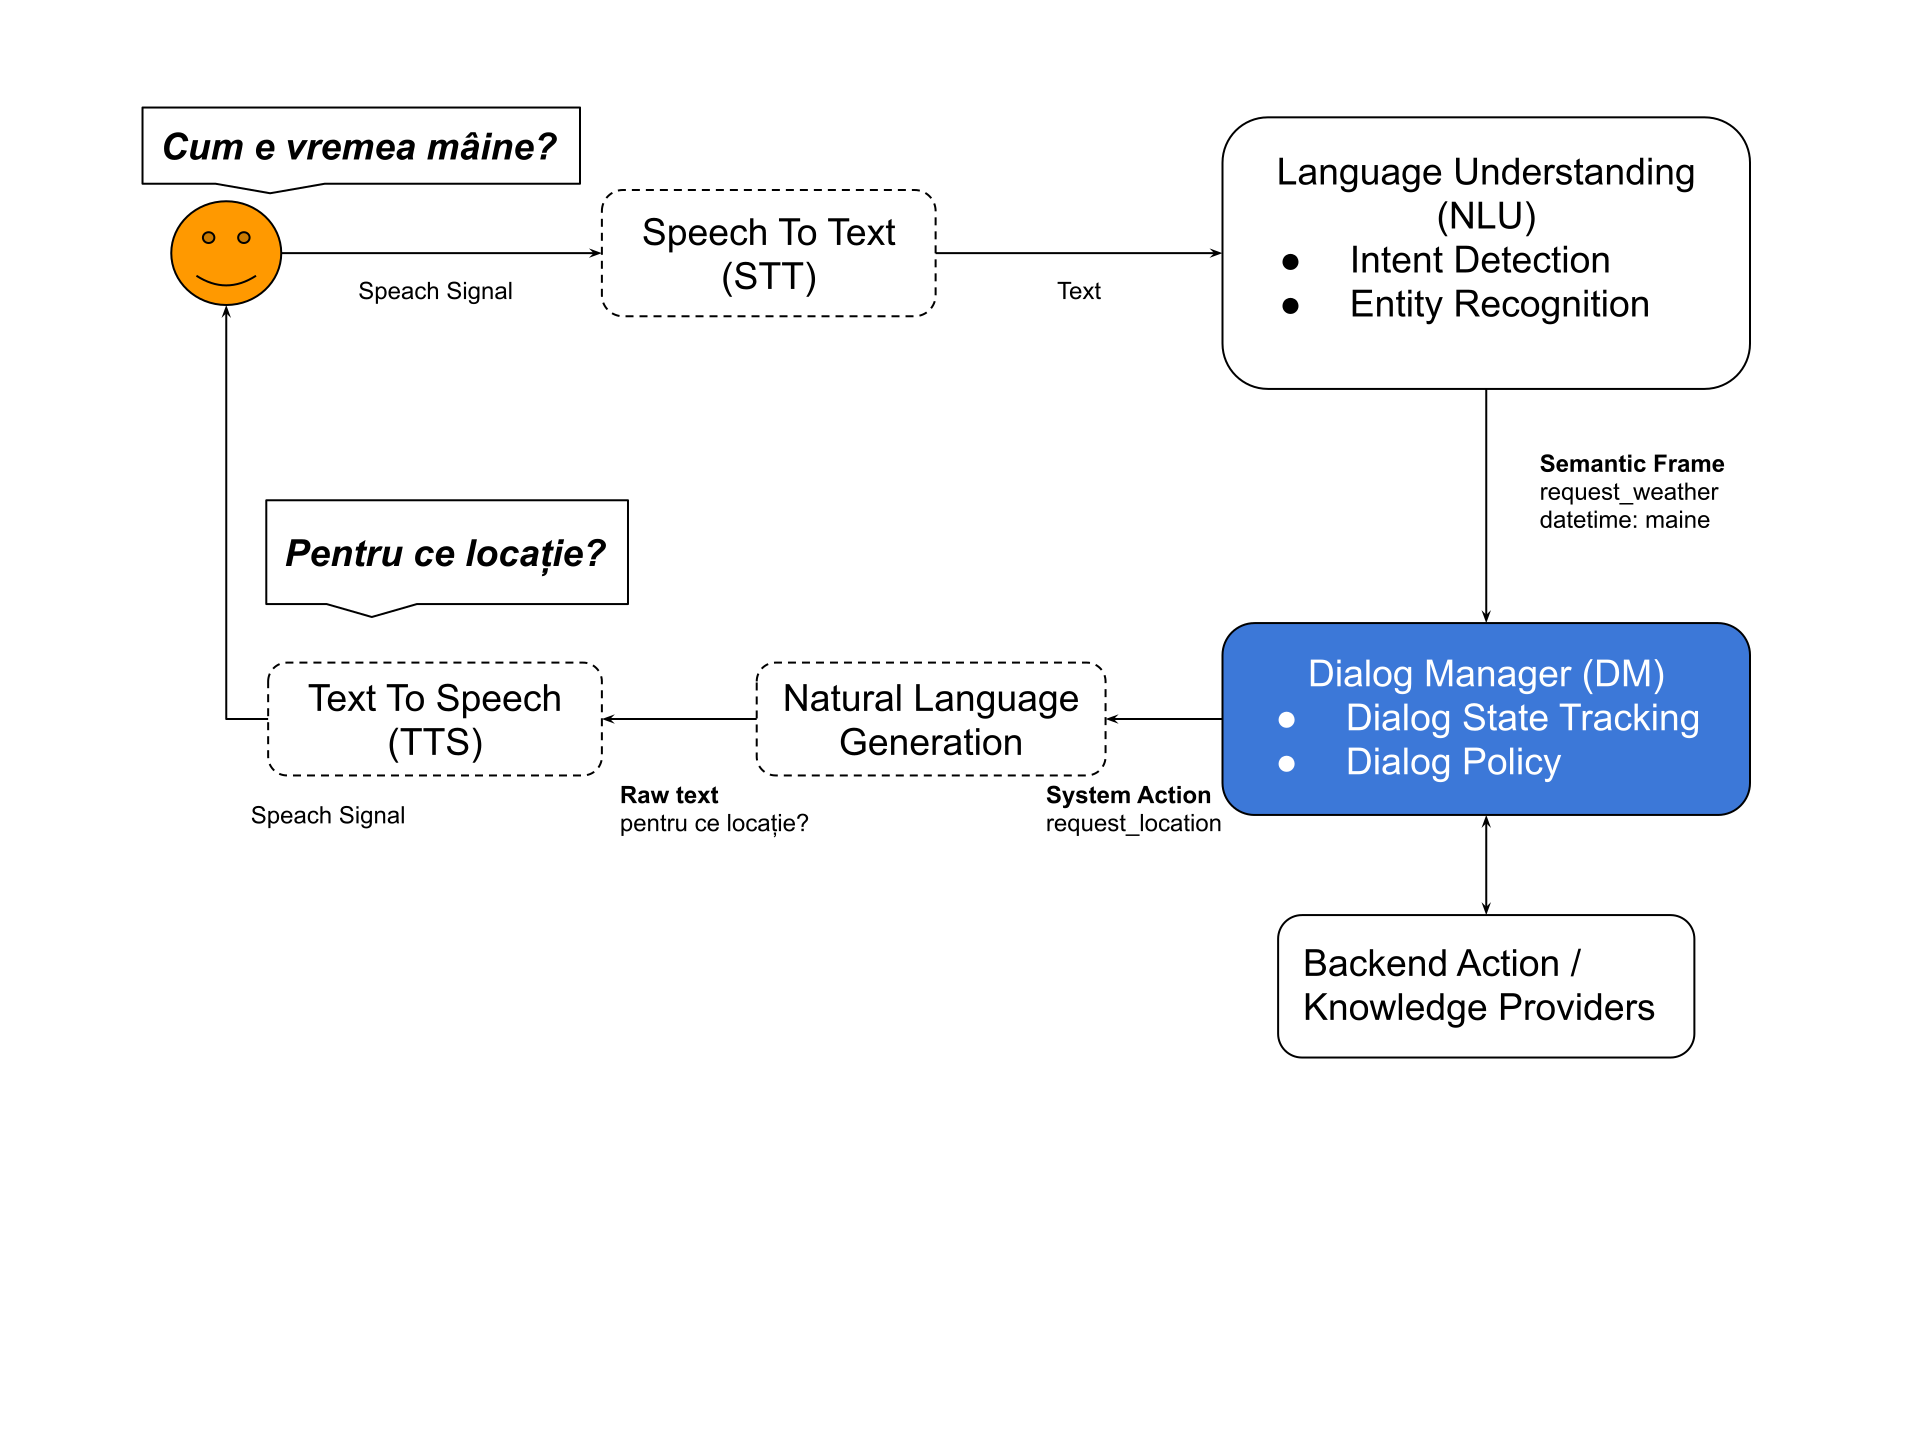
\includegraphics[scale=0.3]{dm_dialog_system.png}
	\caption{Administrator de dialog}
	\label{fig:dm_ds_proc}
\end{figure}

Într-un sistem de dialog au loc mai multe schimburi de informații între utilizator și agent. Acest flux de date nu poate exista fără context, limbaj comun, intenții, entități și nu în ultimul rând acțiuni de ambele părți. Partea responsabilă de înțelegerea limbajului natural ne oferă un cadru semantic compus din intenție și entități la fiecare replică a utilizatorului. Administratorul de dialog este unitatea centrală care coordonează activitatea celorlalte componente, el se folosește de anumite politici pentru a știi ce acțiuni să facă mai departe știind contextul actual.

Două procese importante au loc aici și anume reprezentarea contextului și inferența responsabilă de următoarea acțiune luată de agent.
Ca urmare a acțiunilor sale putem avea interogări ale sistemelor externe, întrebări suplimentare sau notificări privind starea unui anumit obiectiv.
De asemenea tot el se ocupă cu situațiile neclare sau cu cazurile aflate în afara competenței sistemului.

\subsection{Abordări anterioare}

De-a lungul timpului s-a propus diferite abordări de a gestiona dialogul, majoritatea reprezintă contextul conversației ca o stare a dialogului ce persistă într-o structură de date și utilizează diferite mecanisme de decizie pentru a selecta acțiunea corectă. În continuare se vor prezenta pe scurt unele dintre cele mai folosite abordări de a gestiona dialogul.

\textbf{Automat finit determinist - Finite State Automata}\\
Această metodă este ce mai simpla și cea mai întâlnită, ea presupune ca stările unui dialog să fie chiar stările unui automat finit, iar tranzițiile să se realizeze pe baza unor condiții stabilite. Avantajul acestei metode il reprezintă în sine determinismul dat de automat, pentru că în majoritatea cazurilor practice se dorește un comportament stabil, a cărui fir de decizie să fie ușor de despicat. Dezavantajul este acela că agentul va avea întotdeauna inițiativa dialogului, lucru ce descrie o conversație nu în tocmai naturală.
	
\textbf{Cadru de informații - Frame based/Slot filling}\\
Metoda impune schematizarea unui scenariu de dialog într-o structură tabelară. Ea mai este întâlnită și sub denumirea de umplere de sloturi. Un slot este o entitate semantică văzută ca un argument ce va fi umplut de modulul de NLU, iar apoi când au fost umplute suficiente sloturi, are loc acțiunea din partea administratorului de dialog. Altfel spus un cadru de informație este compus din sloturi necesare și un obiectiv al utilizatorului. În mare parte această abordare captează strategia de bază al unui agent, scutind munca depusa pentru a același comportament descris într-un automat finit, ba mai mult dă o flexibilitate dezvoltării datorită structurii tabelare ce poate fi importată. Un alt avantaj este acela că inițiativa la discurs se găsește într-un echilibru, utilizatorul având posibilitatea să ofere mai multe sloturi în aceeași replică. Faptul că suntem constrânși la un singur scenariu reprezintă un dezavantaj.

\textbf{Plan}\\
Abordările bazate pe un plan tratează fiecare replică din dialog ca o acțiune din partea utilizatorului spre a-și atinge obiectivul. Agentul detectează intenția, apoi construiește un plan de comunicare pentru a-l ajuta pe interlocutor să își atingă scopul.

\textbf{Învățare de strategii}\\
Datorită recentelor descoperiri în procesarea limbajului natural \cite{metode-de-reprezentare} și a progreselor din învățarea automată \cite{rnn}, reprezentarea informației și inferența au devenit din ce în ce mai performante. Ceea ce coincide cu necesitățile unui sistem de dialog unde știm ca avem nevoie de o metodă care să poată reprezenta contextul și încă una de a rezona pe baza acestuia. De aici și numărul mare de lucrări științifice în această direcție.

În abordările de acest gen se pleacă de la aceleași principii și anume o mulțime de stări ale conversației și o altă mulțime de acțiuni pe care agentul le poate efectua. Privind conversația ca un proces parțial observat putem atașa un model statistic (partially observable Markov decision process - POMDP), care să ne permită o tranziție din starea A în starea B pe baza unei probabilități.

Avantajele acestor metode sunt legate de automatizarea dezvoltării unui administrator de dialog. Învățarea politicilor de decizie se realizează doar pe baza interacțiunilor anterioare dintre utilizatori și agent. Îmbunătățiri se observă și în calitatea conversației, deoarece antrenarea recompensează conversațiile încheiate cu succes și care durează mai puțin (ca număr de replici). Un plus este adus și în gestionarea situațiilor neprevăzute, ceea ce nu găsim la metodele deterministe descrise anterior.

Puterea oferită de aceste abordări vine și cu costuri: mulțimi de antrenare mai mari - detaliate la nivel de conversație și antrenarea într-un mediu ce simulează utilizatorul final. Bineînțeles faza de învățare poate avea loc și online, dar iar ne vom lovim de lipsa datelor, mai presus de atât expunerea unui agent neantrenat, riscă să deranjeze majoritatea utilizatorilor care au sosit în sistem pentru o cu totul altă problemă.

\subsection{Model propus}

Scopul dezvoltării agenților conversaționali este de a îmbunătății interacțiunea dintre oameni și tehnologie. Prin caracterul său natural, această conexiune impune standarde ridicate în experiența utilizatorului și în eficiența de a rezolva cerințele acestuia. Luând în considerare fragilitatea unui dialog, dar și legătura dintre comportamentul agentului și calitatea conversației, de cele mai multe ori se recurge la implementări bazate pe reguli. Una dintre cela mai populare este cea bazată pe umplerea de sloturi (cadru de informații) care se caracterizează prin următoarele avantaje:
\begin{itemize}
	\item inițiativa la discurs se găsește într-un echilibru, astfel utilizatorul nu se mai simte ghidat ca într-un formular ci mai degrabă într-o discuție
	\item utilizatorul are posibilitatea să ofere mai multe sloturi în aceeași replică, ceea ce crește semnificativ experiența cu agentul care de data aceasta recunoaște mai multe entități într-o propoziție, evitând pe viitor să mai întrebe despre ale
	\item se vede ușor procesul de decizie, fiind un model bazat pe reguli ne dă posibilitatea să mergem pe fir înapoi și să identificăm ipotezele unor anumite acțiuni
	\item comportament previzibil, o oarecare robustețe este impusă atunci când dorim să avem control asupra sarcinilor gestionate
	\item ușor de importat scenarii noi
	\item nu necesită mulțimi de antrenare la fel de bine construite precum modelele statistice, aici fiind nevoie doar de un expert în domeniu care să structureze scenariile de dialog
\end{itemize}

Dezavataje
\begin{itemize}
	\item complexitatea structurii de dialog este proporțională cu numărul de scenarii gestionate, lucru ce limitează această abordare la un număr rezonabil de sarcini
	\item puterea de scalabilitate este legată de competența expertului în domeniu	
\end{itemize}

O îmbunătățire adusă metodei standard de umplere a sloturilor o reprezintă capacitatea de a trata obiective multiple.
Pentru dezvoltarea administratorului de dialog, s-a folosit un model bazat pe cadre de informații (frame based/slot filling) ce poate trata mai multe obiective.
Pentru a ține evidența intențiilor și entităților se folosește o bază de date care descrie aceste concepte, ea poartă numele de ontologie a domeniului și este folosită în comun de componentele de NLU și DM pentru a asigura consistența cerută în comunicarea celor două. Vezi anexa x

Structura dialogului este o altă sursă de date care indică administratorului de dialog logica scenariilor posibile și obiectivele/sarcinile gestionate de către agent. În acest caz sarcină este sinonim cu obiectiv, deoarece ele se referă într-un final la același concept. Astfel un obiectiv al utilizatorului devine o sarcină a sistemului. Deci vorbind din perspectiva consumatorului, un obiectiv este o structură ce pune la o laltă intenția și entitățiile necesare pentru ca acel obiectiv să poată avea loc.

Administratorul de dialog este format din două componente: 
\begin{description}
	\item[Gestionarea stării conversației (Dialog state tracking)] care ține istoria sesiunii de dialog grupată în intenții și entități menționate. Conform structurii de dialog această componentă reușește să mențină o evidența a obiectivelor pe parcursul întregii conversații.
	\item[Politicile de decizie (Dialog policy)] sunt metode/regulile prin care agentul decide să facă anumite acțiuni, de exemplu să întrebe despre un slot lipsă sau să interogheze sistemul rezolvând o anumită sarcină.
\end{description}



